\documentclass{article}
\usepackage{graphicx}
\usepackage{hyperref}

\graphicspath{ {.} }

\title{Python pour la sécurité}
\date{10 aput 2021}
\author{Arthur Saint-Denis}


\begin{document}

\maketitle

\section*{Timing attack}
\subsection*{Définition}

Le principe d'une attaque sur le timing est de récupérer des informations  à partir du temps que met une requête à se compléter.

L'attaque que nous allons essayer de réaliser ici repose sur le fait que 
la comparaison de strings est, par défaut sensible à ce genre d'attaque, dans la plupart des languages.
Lorsque deux strings sont comparés character par character, la comparaison s'arrête dès qu'un character différent est trouvé. Donc comparer deux strings similaires prendra légèrement plus de temps que comparer des strings complètement différentes.

On pourrait donc \emph{en théorie} trouver un mot de passe lettre par lettre en essayant l'une après l'autre toutes les lettres possibles et en gardant celle qui met le plus de temps à être comparée.

Nous avons donc un serveur (cf. server.py, server.go) avec un endpoint /admin/login qui renvoie le status 200 si le mot de passe passé dans le corps de la requête est le bon et 401 si il est mauvais.

\subsection*{Tests préliminaires}

Avant de se lancer dans l'attaque j'ai effectué un test (cf. fichier test\_attack\_vector.py) dans lequel je compare une requête faite au serveur contenant le mot de passe correct avec une requête contenant le mauvais mot de passe. Cela nous permettra d'obtenir des différences de temps maximales.

\begin{center}
    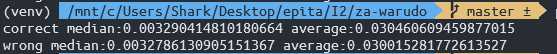
\includegraphics[scale=0.8]{attack_results.png}
\end{center}

On constate vite (après 100 000 requêtes par mot de passe) que le temps de réponse en moyenne (et médian) de la requête contenant le bon mot de passe est plus long.

J'ai ensuite tracé les résultats sur un graphe:

\begin{figure}
    \caption{Serveur Flask}
    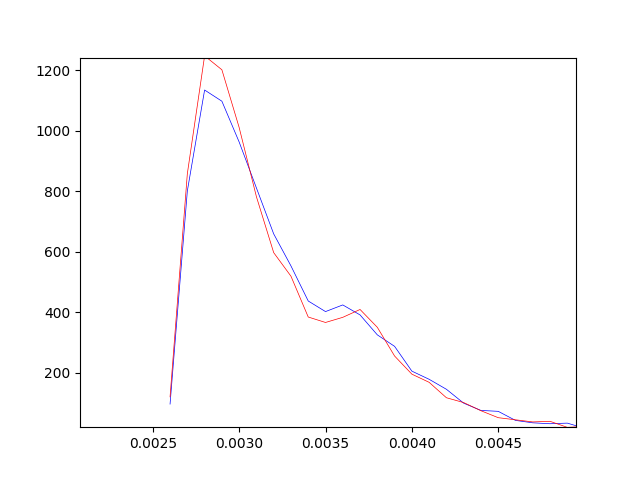
\includegraphics[scale=0.6]{results_plot.png}
\end{figure}


Les figures 1 et 2 représentent le graphe du nombre de requêtes en fonction du temps pris, avec les requêtes corrects en bleu et les requêtes incorrectes en bleu.

La figure 1 provient d'un serveur flask, tandis que la deuxième provient d'un serveur écrit en go, qui est plus rapide et plus constant dans les temps de réponse et permet des résultats plus précis.

On constate que même si il arrive que des requêtes avec le mauvais mot de passe aillent plus vite que des requêtes avec le bon mot de passe, en général, celles-ci sont plus lentes.

\begin{figure}
    \caption{Serveur Go}
    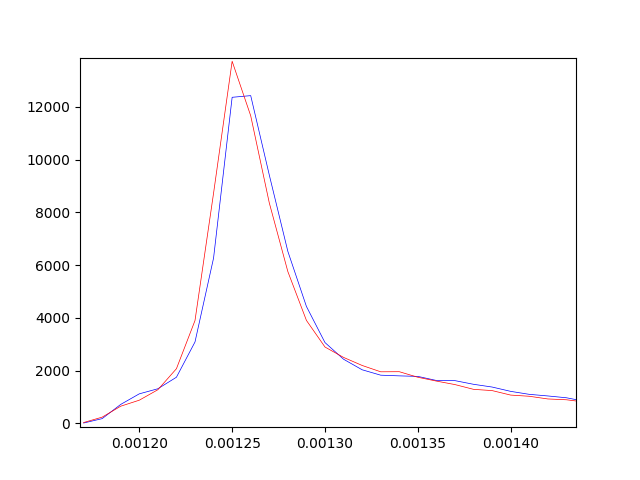
\includegraphics[scale=0.6]{results_plot_go.png}
\end{figure}

Maintenant que l'on sait qu'il y'a une différence dans les temps de comparaison de mots de passe, on peut \emph{essayer} de trouver le mot de passe character par character.

\subsection*{L'attaque}

Le principe reste le même, on compare les temps d'execution character par character et on continue l'attaque avec le character pour lequel le serveur a mit le plus de temps à répondre.

Pour simplifier les choses, je vais utiliser un mot de passe uniquement constitué des lettres a, b et c, mais le principe reste le même pour un alphabet plus grand.

Pour éviter d'avoir trop de différence entre chaque essai, je ne vais pas essayer 100000 fois la lettre a, puis 100000 la lettre b, etc... mais plutôt essayer une fois la lettre a, puis une fois la lettre b puis une fois la lettre c en boucle. Ainsi si, par exemple mon réseau ralentit, il sera ralenti pour les trois lettres et non pas pour une seule, ce qui pourrait fausser les résultats.

Malheureusement, après plusieurs essais, je constate que l'attaque finit systématiquement par se tromper sur une des lettres. A partir de là, tout le reste de l'attaque est faussé.

Je suppose que cela est du au fait que la comparaison d'un seul character se fait beaucoup trop rapidement pour que mon attaque soit consistante.

\begin{figure}
    \caption{Attaque échouant après 5 characters corrects}
    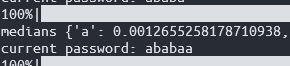
\includegraphics{echec.png}
\end{figure}

\subsection*{Conclusion}

Je n'ai pas été en mesure de réaliser une attaque complète. Mais cela pourrait être possible avec quelques améliorations.
Je pense tout d'abord que si mon attaque était capable de détecter une erreur pour pouvoir revenir en arrière, elle pourrait progresser plus qu'elle ne le fait actuellement. Cela pourrait se faire en comparant les temps de réponse actuels avec les temps de réponse précédents.

En plus de cela, je pense qu'en augmentant le nombre d'itérations, les erreurs seraient moins fréquentes.

Je pense que la vulnérabilité causée par la comparaison de strings est dangereuse car elle est très facile à introduire. Heureusement il est facile de s'en prémunir. Certains languages possèdent des fonctions de comparaison qui sont plus robustes, par exemple: Node.js possède 
\href{https://nodejs.org/api/crypto.html\#cryptotimingsafeequala-b}{crypto.timingSafeEqual} et python possède \href{https://docs.python.org/3/library/hmac.html\#hmac.compare\_digest}{hmac.compare\_digest}. En plus de cela, une telle attaque serait particulièrement longue à réaliser.
Enfin, dans un contexte plus crédible, cette attaque ne permettrait que de récupérer des hashs de mots de passe, ce qui est tout de suite moins intéressant.

\end{document}